%-----------------------------------------------------------------------------------------
\clearpage
\section{Background Research}
%-----------------------------------------------------------------------------------------

In this section, a literature review is firstly introduced to present the most relevant works to this project. In the second part, previous systems in similar project is introduced. The third part provides an detailed analysis of the data characteristics.

\subsection{Literature Review}
This section introduced principles and techniques for data preprocessing and text data visualization.

Text Visualisation Browser \cite{Kucher2014} is an online tool providing the most comprehensive summary of published text visualization \cite{Cao2016}. According to Text Visualisation Browser, from 1976 to 2017, there are 400 published text visualisation papers in total, in which 396 publications are aim to analyse text alignment. By searching "Word", there shows 20 publications, and "Translation" gets 16 results. Whereas when typing "Frequency" and "Weighting", each key word get 1 results. Also, key words such as "Machine learning, "Data Mining", "Natural Language Processing" got no publication collected. The results indicate that in text visualization domain, most researches focus on presenting alignment of texts. There are certain amounts of research focus on the topic such as "word analysis" and "translation", which is similar with this project. However, applying more specific techniques such as "Natural Language Processing" haven't been applied in text visualisation widely.


\paragraph{Interactive Exploration of Versions across Multiple Documents}

\paragraph[]{}Work of \cite{Jong2008} provide a interactive visualization tool, MultiVersioner, to address the issues of comparing several versions of texts.

\paragraph{Visualizations for Text Re-use}

\paragraph[]{}

\paragraph{Interactive Visual Alignment of Medieval Text Versions}

\paragraph[]{}

\paragraph{Design Rules for Visualizing Text Variant Graphs}

\paragraph[]{}

\paragraph{ShakerVis: Visual Analysis of Segment Variation of German Translations of Shakespeare’s \emph{Othello}}

\paragraph[]{}

\paragraph{Visualizations Translation Variation of Shakespeare's Othello: A Survey of Text Visualisation and Analysis Tools}

\paragraph[]{}

\subsection{Previous Systems}

The Version Variation Visualization (VVV) project was introduced by Dr Tom Cheesman from Modern Language Centre at Swansea University. It aims to create interactive data visualization system to build cross-cultural exploration networks. The VVV project focus on developing digital tools which can help to compare and analyze different versions of translation \cite{Cheesman2012}. So far, the tools developed in the project is Ebla, Prism and ShakerVis. Ebla, served as the copus, is a software to stock the text data and detailed information of them. Prism provides the interface for separating texts into segments and processing the segments as alignment. Based on the idea of these two software, ShakerVis provides an interactive interface for visualizing the information of the translation versions \cite{Geng2015}.

There are three types of data visualization in this project: Time-Map, Alignment Maps, Parallel view and Eddy and Viv view. 

\paragraph{Time-Map}
\paragraph[]{}

Figure \ref{fig:timeMap} provides a screen shot of Time Map, which shows the location of the authors and the year of translation versions published. From this view, we can tell that some particular places such as Berlin and Dresden

\begin{figure}[h] 
	\centering	
	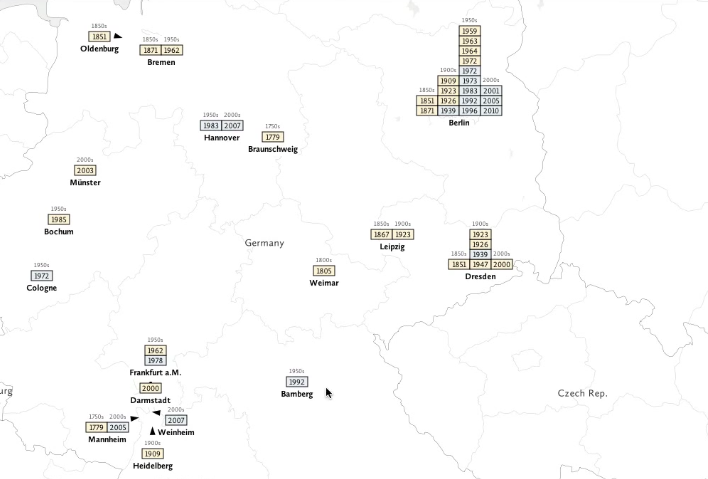
\includegraphics[width=16cm, height=14cm]{Figs/Time-Map}\\[1ex]
	\caption{Time-Map provides an interactive overview of the corpus meta data (\cite{Cheesman2012})}
	\label{fig:timeMap}
\end{figure} 

\paragraph{Alignment Map}
\paragraph[]{}

Figure \ref{fig:alignmentMap} exhibits a structure visualization which compares the segments of the texts between base text and translation versions. By comparing these texts, one can tell the general difference and variation between the base text and translations. For example, if one paragraph of several translations is longer than that of the base text, it is possible that particular expression of German is more complex or detailed than the English. 

\begin{figure}[h] 
	\centering	
	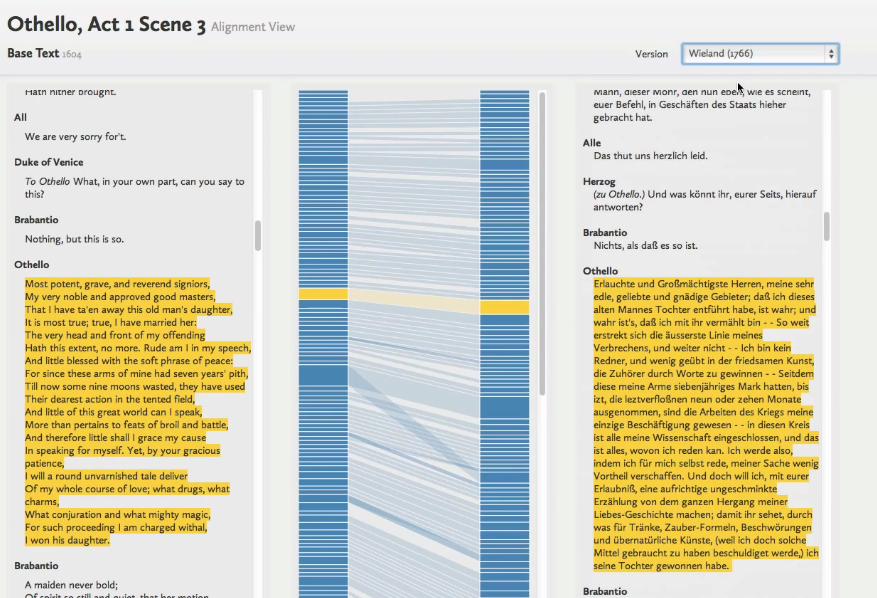
\includegraphics[width=16cm, height=14cm]{Figs/Alignment-Map}\\[1ex]
	\caption{Alignment Maps provides an comparative visualiztion of segments (\cite{Cheesman2012})}
	\label{fig:alignmentMap}
\end{figure} 

\paragraph{Parallel View}
\paragraph[]{}

Figure \ref{fig:parallelView} shows a straightforward view between base text and selected translations. In this visualization, segments are more explicit to find.

\begin{figure}[h] 
	\centering	
	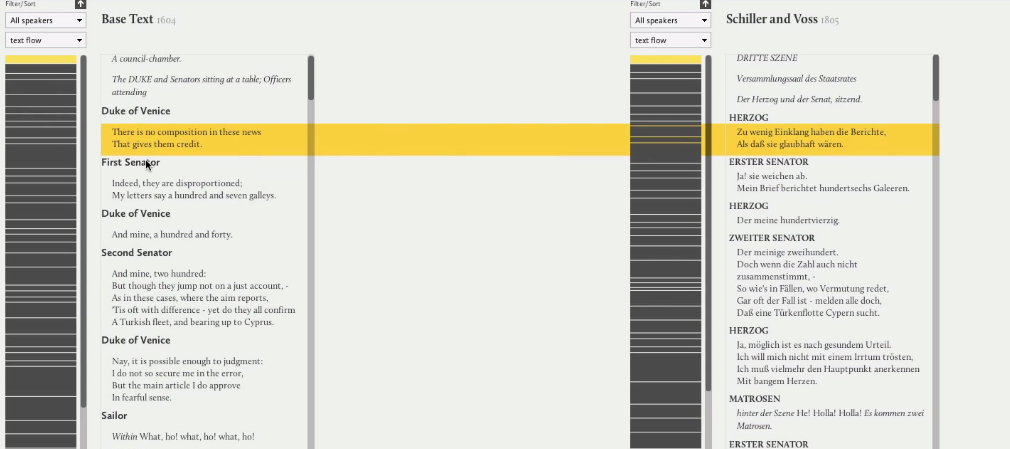
\includegraphics[width=16cm, height=14cm]{Figs/Parallel-View}\\[1ex]
	\caption{Parallel View provides an explicit view between the base text and selected version (\cite{Cheesman2012})}
	\label{fig:parallelView}
\end{figure} 

\paragraph{Eddy and Viv View}
\paragraph[]{}

Figure \ref{fig:eddyVivView} shows Eddy and Viv view, which provides more information of the translation comparison. From the sort bar, we can tell that there are four types can be visualized. Eddy value shows the variation of words used in segment. Relatively, Viv value provides the changes or rivalries for some segments in translation. If we choose version name, segment length or reference date as the order of sorting, there will be other information of translation variations. Also, there are backtranslation based on machine translation provided, which is another powerful function for comparing the text data.

\begin{figure}[h] 
	\centering	
	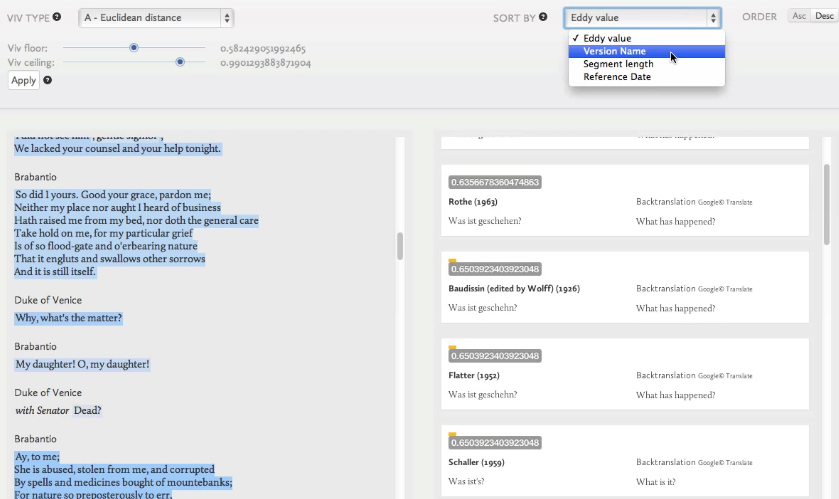
\includegraphics[width=16cm, height=14cm]{Figs/Eddy-Viv-View}\\[1ex]
	\caption{Eddy and Vis view enable researchers to understand more details of vocabulary (\cite{Cheesman2012})}
	\label{fig:eddyVivView}
\end{figure} 



